\section{An\'alisis}

\subsection{Descripci\'on}
Este prototipo se encarga de la toma de desiciones del clasificador de nivel 5 y el clasificador de niveles  1, 2, 3, 4 y 6.

\subsection{Objetivo}
Desarrollar el API de decisi\'on a partir de la uni\'on de los clasificadores de nivel 5 y niveles 1, 2, 3, 4 y 6.

\subsection{Caracter\'isticas}
\begin{description}
\item[FEAT1:] La API recibe como entrada conversaciones en archivos de texto plano.
\item[FEAT2:] La API recibe como entrada conversaciones en archivos con formato xml.
\item[FEAT4:] La API preprocesa textos.
\item[FEAT4:] La API genera vectores de nivel 5.
\item[FEAT5:] La API genera vectores de nivel  1, 2, 3, 4 y 6.
\item[FEAT6:] El API dar\'a como salida la decisi\'on del clasificador dle prototipo4.

\end{description}

\subsection{Restricciones}
\begin{itemize}
\item Prototipo programado en lenguaje Python versi\'on 2.7.
\end{itemize}



\section{Dise\~no}


\section{Arquitectura}

La figura \ref{fig:arquitecturap5} muestra la arquitectura de la API de an\'alisis.

\begin{figure}[h]
\begin{center}
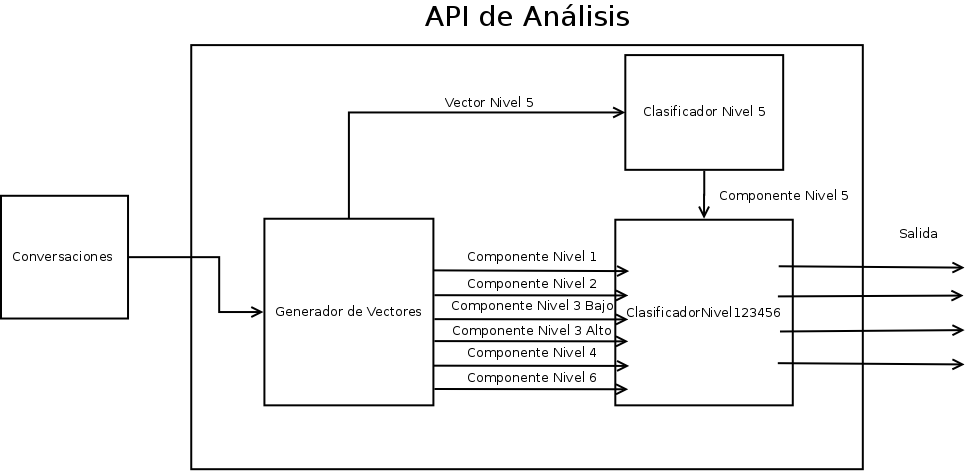
\includegraphics[scale=.3]{images/api}
\caption{Arquitectura de la API de an\'alisis}
\label{fig:arquitecturap5}
\end{center}
\end{figure}


\subsection{Diagrama de clases}


La figura \ref{fig:dclasesp5} muestra el diagrama de clases de la API de an\'alisis.
\begin{figure}[h]
\begin{center}
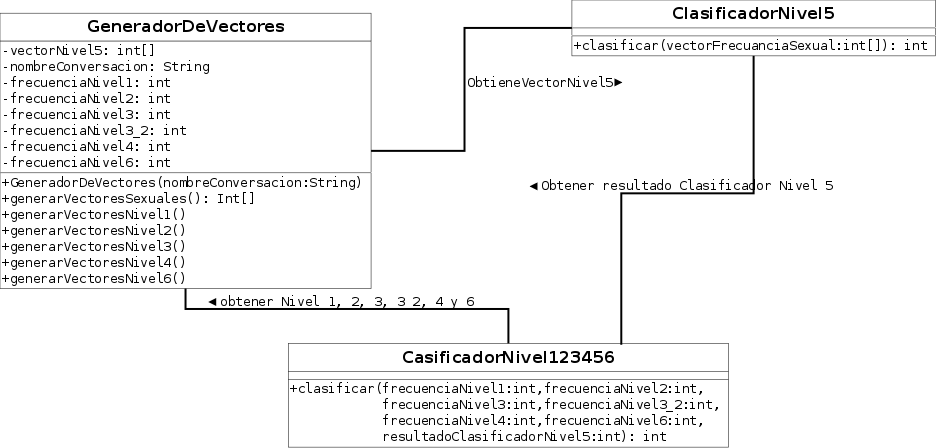
\includegraphics[scale=.3]{images/api2}
\caption{Diagrama de clases de la API de an\'alisis}
\label{fig:dclasesp5}
\end{center}
\end{figure}

Como se puede observar en el diagrama de clases de la figura \ref{fig:dclasesp5}, el sistema consta de 3 clases:


\subsubsection{Clase: GeneradorDeVectores}
Descripci\'on: Esta clase produce los vectores de las incidencias de las frases de los niveles 1, 2, 3, 3\_2, 4 y 6 encontradas dentro de las conversaciones.
Atributos: 
\begin{description}
\item[vectorNivel5]: Vector que representa la existencia de incidencias de palabras de car\'acter sexual dentro de la conversaci\'on.
\item[nombreConversacion]: Nombre del archivo de la conversaci\'on.
\item[frecuenciaNivel1]: Entero que representa el n\'umero de incidencias de frases de Nivel 1 (Amistad). 
\item[frecuenciaNivel2]: Entero que representa el n\'umero de incidencias de frases de Nivel 2 (Relaci\'on).
\item[frecuenciaNivel3]: Entero que representa el n\'umero de incidencias de frases de Nivel 3 (Riesgo).
\item[frecuenciaNivel3\_2]: Entero que representa si la frecuencia de incidencias de Nivel 3 es excesiva.
\item[frecuenciaNivel4]: Entero que representa el n\'umero de incidencias de frases de Nivel 4 (Exclusividad).
\item[frecuenciaNivel6]: Entero que representa el n\'umero de incidencias de frases de Nivel 5 (Conclusi\'on).
\end{description}

M\'etodos:
\begin{description}
\item[generarVectoresSexuales]: Este m\'etodo se encarga de generar el vector que representa las incidencias de palabras de car\'acter sexual.
\item[generarVectoresNivel1]: Este m\'etodo se encarga de generar el vector que representa las incidencias de frases de Nivel 1 (Amistad).
\item[generarVectoresNivel2]: Este m\'etodo se encarga de generar el vector que representa las incidencias de frases de Nivel 2 (Relaci\'on).
\item[generarVectoresNivel3]: Este m\'etodo se encarga de generar el vector que representa las incidencias de frases de Nivel 3 (Riesgo).
\item[generarVectoresNivel4]: Este m\'etodo se encarga de generar el vector que representa las incidencias de frases de Nivel 4 (Exclusividad).
\item[generarVectoresNivel6]: Este m\'etodo se encarga de generar el vector que representa las incidencias de frases de Nivel 6 (Conclusi\'on).
\end{description}

\subsubsection{Clase: ClasificadorNivel5}
Descripci\'on: Esta clase categoriza el vector de frecuencia sexual en peligroso y no peligroso dependiendo de si GeneradorDeVectores encontr\'o alguna incidencia de car\'acter sexual dentro de la conversaci\'on.  
M\'etodos:
\begin{description}
\item[clasificar]: Este m\'etodo genera un entero que representa la existencia o no existencia de palabras de car\'acter sexual dentro de la conversaci\'on. 
\end{description}

\subsubsection{Clase: ClasificadorNivel123456}
Descripci\'on: Esta clase categoriza el vector recibido en 4 niveles distintos: No Peligroso, Poco Peligroso, Peligroso y Muy Peligroso.

M\'etodos:
\begin{description}
\item[clasificar]: Se encarga de categorizar si el vector resultante es No Peligroso, Poco Peligroso, Peligroso o Muy Peligroso con base en la matriz de entrenamiento.
\end{description}

\section{Pruebas}


%La tabla  \ref{tab:resultadasapi} muestra la tabla de resultados de conversaciones nuevas y su respectivo resultado.
%
%\begin{table}
%\begin{center}
%
%
%\begin{tabular}{|l|c|c|c|c|c|c|c|c|}
%
%\hline
%Conversaci\'on & N1 & N2 & N3 & N\_3 & N4 & N5 & N6 & Decisi\'on \\
%\hline
%pruebas/pr10.txt &
% 0 &
% 3 &
% 0 &
% 0 &
% 0 &
% 1 &
% 1 &
%Muy Peligrosa \\
%pruebas/pr11.txt &
% 0 &
% 4 &
% 0 &
% 0 &
% 0 &
% 1 &
% 0 &
%Muy Peligrosa \\ 
%pruebas/pr12.txt &
% 0 &
% 0 &
% 6 &
% 4 &
% 0 &
% 1 &
% 0 &
%Muy Peligrosa \\ 
%pruebas/pr13np.txt &
% 0 &
% 1 &
% 0 &
%  0 &
% 0 &
% 0 &
% 0 &
%No Peligrosa \\ 
%pruebas/pr14.txt &
% 0 &
% 2 &
% 0 &
% 0 &
% 0 &
% 0 &
% 0 &
%No Peligrosa \\ 
%pruebas/pr15.txt &
% 0 &
% 13 &
% 4 &
% 2 &
% 1 &
% 0 &
% 0 &
%Peligrosa \\
%pruebas/pr16.txt &
% 1 &
% 4 &
% 1 &
% 0 &
% 0 &
% 1 &
% 0 &
%Muy Peligrosa \\ 
%pruebas/pr17.txt &
% 1 &
% 0 &
% 0 &
% 0 &
% 1 &
% 1 &
% 0 &
%Muy Peligrosa \\ 
%pruebas/pr18.txt &
% 4 &
% 7 &
% 5 &
% 3 &
% 0 &
% 1 &
% 0 &
%Muy Peligrosa \\ 
%pruebas/pr19np.txt &
% 0 &
% 2 &
% 0 &
% 0 &
% 0 &
% 0 &
% 0 &
%No Peligrosa \\ 
%pruebas/pr1.txt &
% 2 &
% 10 &
% 0 &
% 0 &
% 1 &
% 1 &
% 3 &
%Muy Peligrosa \\ 
%pruebas/pr20np.txt &
% 0 &
% 2 &
% 0 & 
% 0 &
% 0 &
% 0 &
% 0 &
%No Peligrosa \\ 
%pruebas/pr21.txt &
% 1 &
% 1 &
% 0 &
% 0 &
% 0 &
% 1 &
% 0 &
%Muy Peligrosa \\ 
%pruebas/pr22.txt &
% 0 &
% 4 &
% 0 &
% 0 &
% 0 & 
% 1 &
% 0 &
%Muy Peligrosa \\ 
%pruebas/pr2np.txt &
% 0 &
% 1 & 
% 1 &
% 0 &
% 0 &
% 0 &
% 0 &
%No Peligrosa \\
%pruebas/pr3np.txt &
% 1 &
% 2 &
% 0 &
% 0 &
% 0 &
% 0 &
% 0 &
%No Peligrosa \\
%pruebas/pr4.txt &
% 0 &
% 1 &
% 0 &
% 0 &
% 0 &
% 1 &
% 0 &
%Muy Peligrosa \\
%pruebas/pr5.txt &
% 0 &
% 0 &
% 0 &
% 0 &
% 0 &
% 1 &
% 0 &
%Muy Peligrosa \\
%pruebas/pr6.txt &
% 0 &
% 1 &
% 3 &
% 1 &
% 0 &
% 1 &
% 0 &
%Muy Peligrosa \\ 
%pruebas/pr7.txt &
% 1 &
% 6 &
% 4 &
% 2 &
% 0 &
% 1 &
% 0 &
%Muy Peligrosa \\ 
%pruebas/pr8.txt &
% 0 &
% 1 &
% 1 &
% 0 &
% 1 &
% 1 &
% 0 &
%Muy Peligrosa \\
%pruebas/pr9.txt &
% 0 &
% 0 &
% 0 &
% 0 &
% 0 &
% 1 &
% 0 &
%Muy Peligrosa \\ 
%pruebas/pr23.txt &
% 1 &
% 2 &
% 0 &
% 1 &
% 0 &
% 0 &
% 0 &
%No Peligrosa \\ 
%pruebas/pr24.txt &
% 0 &
% 1 &
% 0 &
% 0 &
% 0 &
% 1 &
% 1 &
%No Peligrosa \\ 
%pruebas/pr25.txt &
% 0 &
% 0 &
% 0 &
% 0 &
% 0 &
% 1 &
% 0 &
%Muy Peligrosa \\ 
%\hline
%\end{tabular}
%
%\caption{Tabla de resultados de la Api}
%\label{tab:resultadasapi}
%\end{center}
%\end{table}

%En la figura \ref{fig:ClasificacionNiv} podemos observar el resultado de las pruebas realizadas en 25 conversaciones distintas. Los resultados muestran el n\'umero de incidencias de las frases categorizadas anteriormente en los niveles 1, 2 ,3,3\_2, 4 y 6; as\'i como el n\'umero de conversaciones que conten\'ian palagras de car\'acter sexual.
%
%\begin{figure}[h]
%\begin{center}
%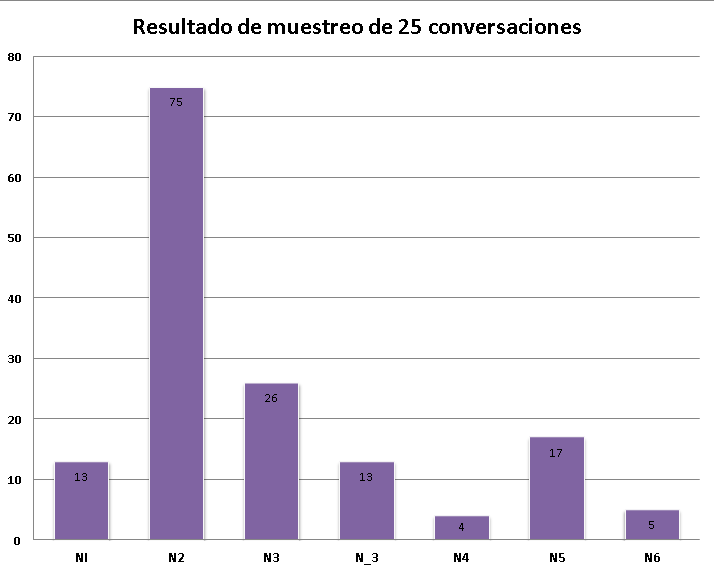
\includegraphics[scale=.7]{images/grafica/ClasificacionNiv}
%\caption{Resultados del muestro de 25 conversaciones}
%\label{fig:ClasificacionNiv}
%\end{center}
%\end{figure}


En la tabla \ref{tab:resultadosM} se muestran los resultados que obtuvimos de las 50 conversaciones anteriormente mencionadas. La tabla contiene el n\'umero de conversaciones que se encontraron de las 4 diferentes categor\'ias: No peligrosa, Poco peligrosa, Peligrosa, Muy peligrosa.

\begin{table}[h]
\begin{center}


\begin{tabular}{|c|c|}
\hline
Clasificaci\'on & Incidencias \\
\hline

No Peligrosa & 23\\
Poco Peligrosa & 0\\
Peligrosa & 1\\
Muy peligrosa & 26\\
\hline
\end{tabular}

\caption{Resultados de muestreo de 50 conversaciones}
\label{tab:resultadosM}
\end{center}
\end{table}

En la figura \ref{fig:ClasificacionConv} podemos observar graficamente la tabla anterior. Los resultados del muestreo de 50 conversaciones muestran que la mayor\'ia de \'estas (17) fueron detectadas como peligrosas.

\begin{figure}[h]
\begin{center}
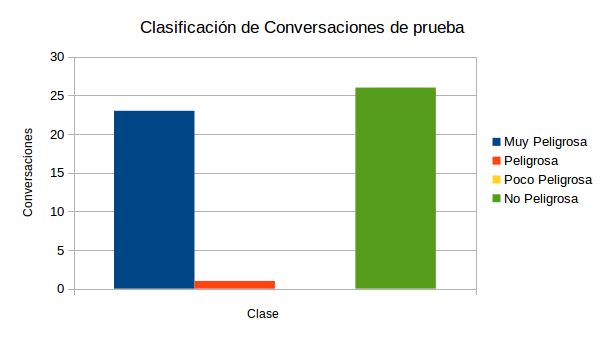
\includegraphics[scale=.7]{images/grafica/ClasificacionConv}
\caption{Resultados del muestro de 25 conversaciones}
\label{fig:ClasificacionConv}
\end{center}
\end{figure}


